% !TeX spellcheck = en_GB
% !TeX root = memoco-report.tex

\section{Introduction}
\label{chap:introduction}

\subsection{Description of the problem}
The task of the exercise was to develop two algorithms capable of solving the Travelling Salesman Problem (TSP), specialized to the domain of drilling holes in electric panels. Given a sequence of holes to be drilled in an electric panel, the algorithms should be used to find a sequence of holes that minimizes the cost of drilling the whole panel, where the costs are given by the euclidean distances between holes. For simplicity it is assumed that the cost of drilling every hole can be ignored.\\ 
The first algorithm implements an exact methods using the IBM CPLEX optimization suite. The second algorithm is an approximated heuristic, inspired by the Lin-Kernighan algorithm \cite{LinK73}. Some implementation details has been taken from \cite{ImplemLK}. \\
Both algorithms have been tested on synthetic instances produced taking into account the applicative domain. The two algorithms are described in the following pages, and tests and results are reported in the last sections.

\subsection{Description of provided material}
%\minitoc
The delivered material includes all the produced code and everything necessary to run the program.
The provided archive comes with the following structure:
\renewcommand*\DTstylecomment{\rmfamily\color{blue}\textit}
\dirtree{%
	.1 /.
	.2 bin/\DTcomment{Binary files folder (after compiling)}.
	.2 build/\DTcomment{Build files folder (after compiling)}.
	.2 files/\DTcomment{Logs folder (after running)}.
	.2 instances/\DTcomment{Contains csv files to load}.
	.2 plots/.
	.2 src/.
	.3 utils/.
	.4 cpxmacro.hpp.
	.4 params.hpp.
	.4 python\_adapter.hpp\DTcomment{Wrapper class for Python embedding}.
	.4 variadic\_table.hpp\DTcomment{Library to print tables}.
	.4 yaml\_parser.hpp\DTcomment{Parser for the configuration file}.
	.3 calibrate.cpp\DTcomment{Calibration script}.
	.3 config.yml.
	.3 CPLEX.cpp.
	.3 CPLEX.hpp.
	.3 LK.cpp.
	.3 LK.hpp.
	.3 main.cpp\DTcomment{Program main}.
	.3 Pair.cpp.
	.3 Pair.hpp.
	.3 plot\_script.py\DTcomment{Script to plot with Python}.
	.3 test.cpp\DTcomment{Test script}.
	.3 Tour.cpp.
	.3 Tour.hpp.
	.3 TSPinstance.cpp.
	.3 TSPinstance.hpp.
	.3 TSPsolution.cpp.
	.3 TSPsolution.hpp.
	.3 utilities.cpp.
	.3 utilities.hpp.
}

\subsubsection{How to run}
The program has the following dependencies:
\begin{itemize}
	\setlength\itemsep{0.03em}
	\item \texttt{g++ 7} or higher;
	\item \texttt{IBM ILOG CPLEX Optimization Studio 12.8} or higher;
	\item \texttt{Python 2.7}.
\end{itemize}

To test the program, some instances should be generated or imported by placing them in the \texttt{instances/} folder. Some files are already provided in this folder to launch some tests. To generate new instances set \texttt{generate\_instances: true} in the \texttt{config.yml} file, and the other parameters as desired. If \texttt{N\_min = 20, N\_incr = 5, N\_max = 30}, three \texttt{csv} files containing the coordinates of every point will be generated, with size 20, 25 and 30 respectively, and will be placed in the instances folder. After that it is possible to run the exact method or the heuristic on these instances. To do that, add to the list in \texttt{instances\_to\_read} the filename (without extension) of the files that should be read and set \texttt{solve\_heur} and \texttt{solve\_cplex} as desired. Some reasonable parameters for the heuristic are already set, but it is possible to change them if necessary. A description of these specific parameters is provided in \cref{ssec:hyperpar}.
The script can then be run from a Linux environment with \texttt{make \&\& ./bin/main}. The algorithm writes its output in file \texttt{solLK.txt} and \texttt{solCPLEX.txt} under the \texttt{files/} folder. When solving more than one problem, these files can also be checked while the program is running to monitor its execution. Additionally running the heuristic also produces an image of the final solution and places it in folder \texttt{plots/}. Furthermore, running both CPLEX and the heuristic together will produce plots with a comparison of the execution times and error values in the same folder. \\

\subsection{Development environment}
The specifics of the machine used for development, calibration and test of the program are listed in \cref{tab:maspecs}.
\begin{table}[H]
	\caption{Hardware and software specifics}
	\label{tab:maspecs}
	\centering
	\begin{tabular}[t]{ll}
		\rowcolor[HTML]{EFEFEF}
		\textbf{Specific} & \textbf{Value} \\
		OS       & Ubuntu 18.04.4 LTS 64 bit	   \\
		Processor & Intel Core i7-7500U 2.70GHz $\times$ 4     \\
		Main memory  & 16 GB  
	\end{tabular}
\end{table}

\section{Dataset generation}
\label{sec:datasetgen}
In order to test the two algorithms, a procedure to build a synthetic dataset of different sizes has been provided.\\ 
The procedure to generate the TSP instances receives as an input a number $N$ of points (which symbolises holes) and generates $N$ pairs representing the coordinates in space of the points on a $N\times N$ square canvas. These points are distributed in a way to resemble the regularity usually found in the disposition of holes in electric panels.\\ 
To do this the procedure draws some regular polygons with up to $10$ sides. Each polygon is generated independently and may overlap with the others, creating not perfectly regular shapes, but neither a completely random point distribution. An example of such an instance is shown in \cref{fig:dataexample}. All this operations, as well as the function to load already generated instances from \texttt{csv} files, are implemented in \texttt{TSPinstance.cpp}.

\begin{figure}[h]
	\centering
	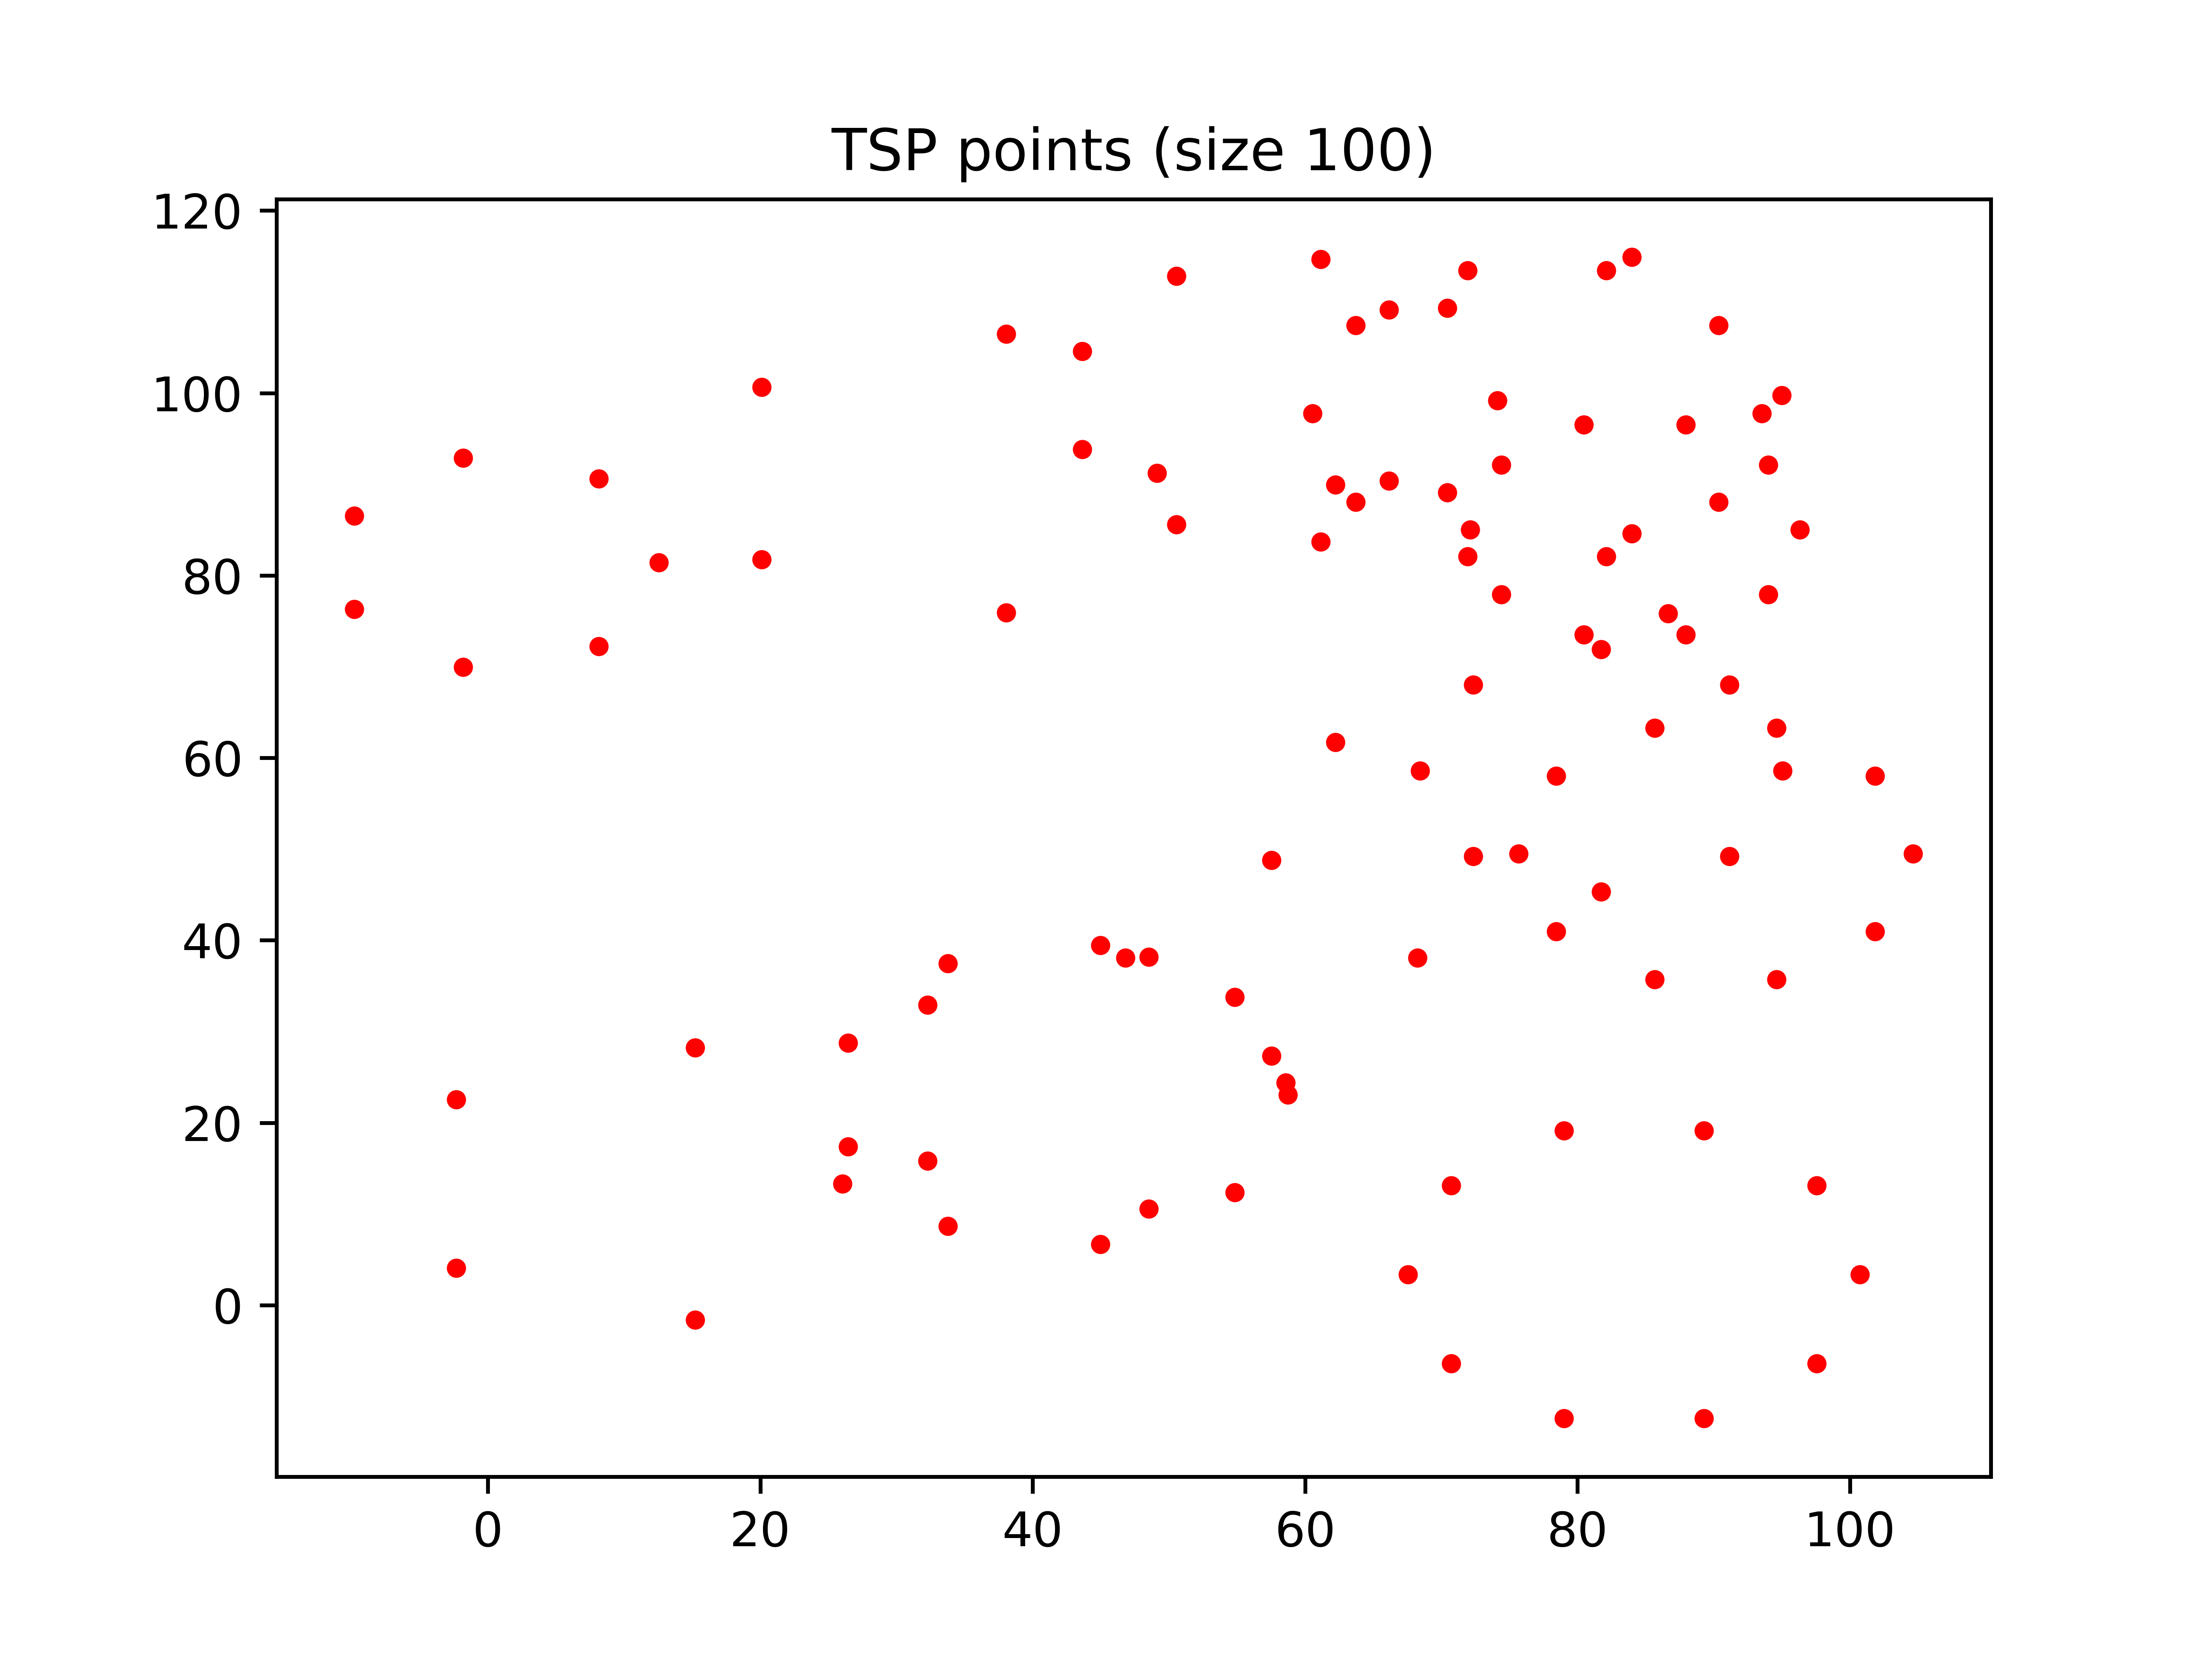
\includegraphics[width=13cm]{path_100}
	\caption{A generated instance of with size N = 100}
	\label{fig:dataexample}
\end{figure}


